\section{Performance Results}
\label{sec:results}

In this section, we present performance results for the MapReduce
graph algorithms of the preceeding section, implemented as small C++
programs calling our MR-MPI library.  The benchmarks were run on a
medium-sized Linux cluster of 2 GHz dual-core AMD Opteron processors
connected via a Myrinet network.  Most importantly for MR-MPI, each
node of the cluster has one local disk, which is used for out-of-core
operations in MR-MPI.  To avoid contention for disk I/O, we ran all
experiments with one MPI process per node.  For comparisons with other
implementations, we used either the same cluster or, where noted,
Sandia's Cray XMT, a multi-threaded parallel computer with 500 {MHz}
processors and a 3D-Torus network.

We ran each of the algorithms on three R-MAT graphs of different
sizes, each on a varying number of processors.  Details of the input
data are shown in Table~\ref{t:rmats}.  The {\it small} problem
(around 8M edges) can typically be run on a single processor without
incurring out-of-core operations.  The {\it medium} problem (around
134M edges) can be run on a single processor with out-of-core
operations; larger processor configurations, however, do not
necessarily require out-of-core operations.  The {\it large} problem
(around 2B edges) requires out-of-core operations on our 64-node
cluster.

%The {\it x-large} problem 
%(around 34B edges) requires most of the machine to run.

All data sets used R-MAT parameters $(a, b, c, d) = (0.57, 0.19, 0.19,
0.05)$ and generated 8 edges per vertex (on average).  These values
create a highly skewed degree distribution, as indicated by the
maximumn vertex degree in Table~\ref{t:rmats}.

\begin{table}
\begin{center}
\begin{tabular}{|l|c|c|c|c|c|c|c|}
\hline
Data & \# of    & \# of & Maximum \\
Set  & vertices & edges & vertex degree\\
\hline
RMAT-20 (small)   &$2^{20} \approx 1M$ & $2^{23} \approx 8M$ &  $\approx 24K$ \\
RMAT-24 (medium)  &$2^{24} \approx 17M$ & $2^{27} \approx 134M$ &  $\approx 147K$ \\
RMAT-28 (large)   &$2^{28} \approx 268M$ & $2^{31} \approx 2B$& $\approx 880K$ \\
%RMAT-32 (x-large) &$2^{32} \approx 4B$ & $2^{35} \approx 34B$ &   \\
\hline
\end{tabular}
\caption{Characteristics of R-MAT input data for graph algorithm
benchmarks.}
\label{t:rmats}
\end{center}
\end{table}

The resulting timings give a sense of the inherent scalability of the
MapReduce algorithms as graph size grows on a fixed number of
processors, and of the parallel scalability for computing on a graph
of fixed size on a growing number of processors.  Where available, we
compare the MapReduce algorithm with other parallel implementations,
including more traditional distributed-memory algorithms and
multi-threaded algorithms in the Multi-Threaded Graph Library
(MTGL)~\cite{MTGL} on the Cray XMT.  We compute parallel efficiency on
$P$ processors as $({time}_{M} \times M) / ({time}_P \times P)$ where
$M$ is the smallest number of processors on which the experiment was
run, and ${time}_I$ is the execution time required on $I$ processors.

\subsection{R-MAT generation results}

In Figure~\ref{f:rmat}, we show the scalability of the R-MAT
generation algorithm (Figure~\ref{fig:rmat2}) for RMAT-20, RMAT-24 and
RMAT-28.  For RMAT-20 and RMAT-24, superlinear speed-up is shown.
This speed-up is due to the decreased amount of file I/O needed with
greater numbers of processors; with a larger total memory, a
fixed-size problem requires less I/O with more processors.  For
RMAT-28, which requires significant out-of-core operations, parallel
efficiency ranges from 52\% to 97\%.  Comparisons between the enhanced
algorithm (Figure~\ref{fig:rmat2}) and the original algorithm
(Figure~\ref{fig:rmat}) showed approximately 10\% reduction in
execution time for the enhanced algorithm.

%Also in Figure~\ref{f:rmat}, we compare our MR-MPI implementation with an 
%R-MAT generator in MTGL on the Cray XMT.  In the MTGL implementation, 
%threads generate edges independently.  A global hash table is used to remove
%duplicate edges.  Our MR-MPI implementation runs more quickly than the MTGL
%implementation.  The differences in execution time are greatest on 64
%processors, where MR-MPI needs the least file I/O for out-of-core operations.

\begin{figure}[htb]
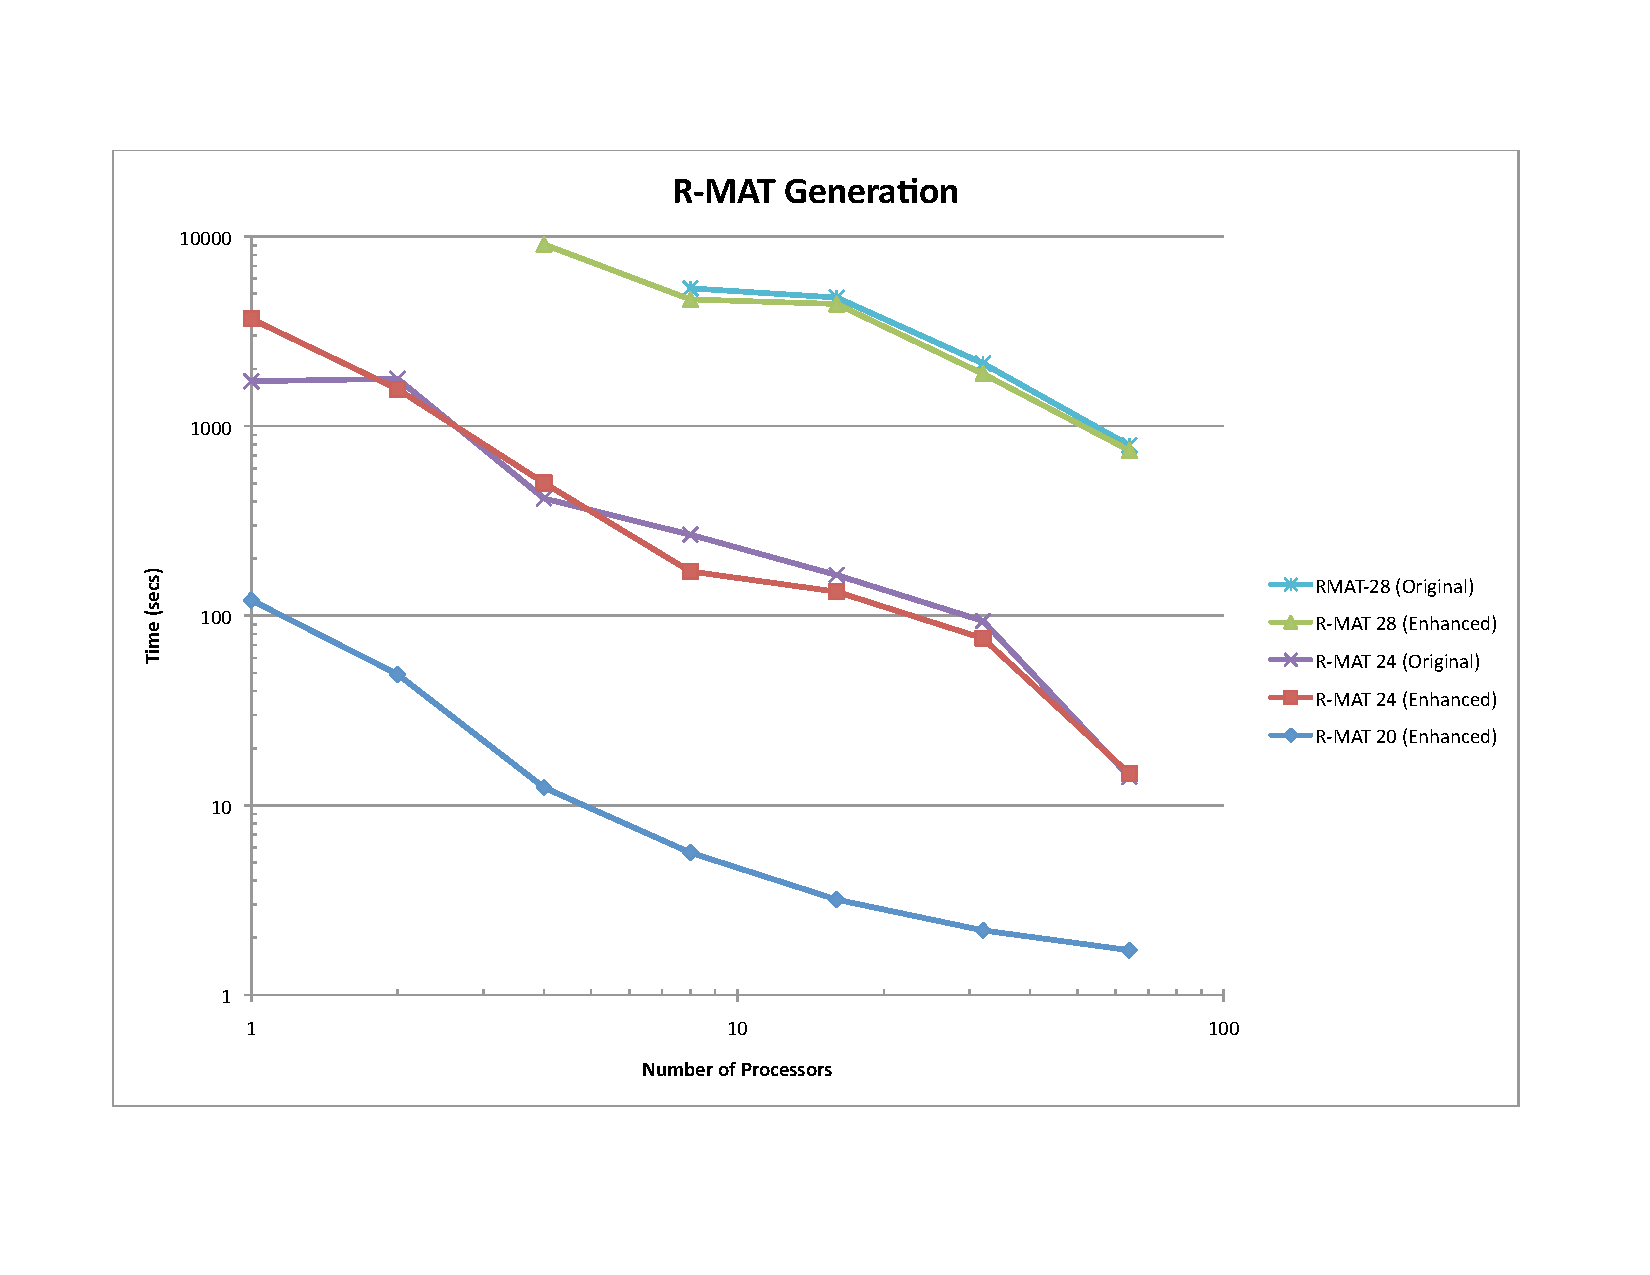
\includegraphics[width=\textwidth]{fig_rmat.pdf}
\caption{Performance of the MR-MPI R-MAT generation algorithm (Figure~\ref{fig:rmat2}) 
%and an MTGL implementation.
}
\label{f:rmat}
\end{figure}

\subsection{PageRank results}
\label{subsec:results_pagerank}

In Figure~\ref{f:pr}, we show the performance of the MR-MPI PageRank
algorithm (Figure~\ref{fig:pr2}) compared to a distributed-memory
matrix-based implementation using the linear algebra toolkit
Trilinos~\cite{Trilinos-Overview}.  The matrix-based
distributed-memory implementation of PageRank uses Trilinos Epetra
matrix/vector classes to represent the graph and PageRank vector.
Rows of matrix $A$ and the associated entries of the PageRank vector
$x$ are uniquely assigned to processors; a random permutation of the
input matrix effectively load balances the non-zero matrix entries
across processors.  Interprocessor communication gathers $x$ values
for matrix-vector multiplication and sums partial products into the
$y$ vector.  Most communication is point-to-point communication, but
some global communication is needed for computing residuals and norms
of $x$ and $y$.

Figure~\ref{f:pr} shows the execution time per PageRank iteration for
R-MAT matrices RMAT-20, RMAT-24 and RMAT-28.  Converging the PageRank
iterations to tolerance $0.002$ requires five or six iterations.
Several R-MAT matrices of each size were generated for the
experiments; the average time over the matrices is reported here.  The
Trilinos implementations show near-perfect strong scaling for RMAT-20
and RMAT-24.  The MR-MPI implementations also demonstrate good strong
scaling.  However, MR-MPI's execution time is at least an order of
magnitude greater than the Trilinos implementation.  
The benefit of MR-MPI's out-of-core implementation
is seen, however, with the RMAT-28 data set, which could be solved on
smaller processor sets than the Trilinos implementation.  For these
experiments, the Trilinos implementation required 64 processors for
the RMAT-28 data set, since it will not operate on matrices that
exceed the aggregate memory of the processors.

\begin{figure}[htb]
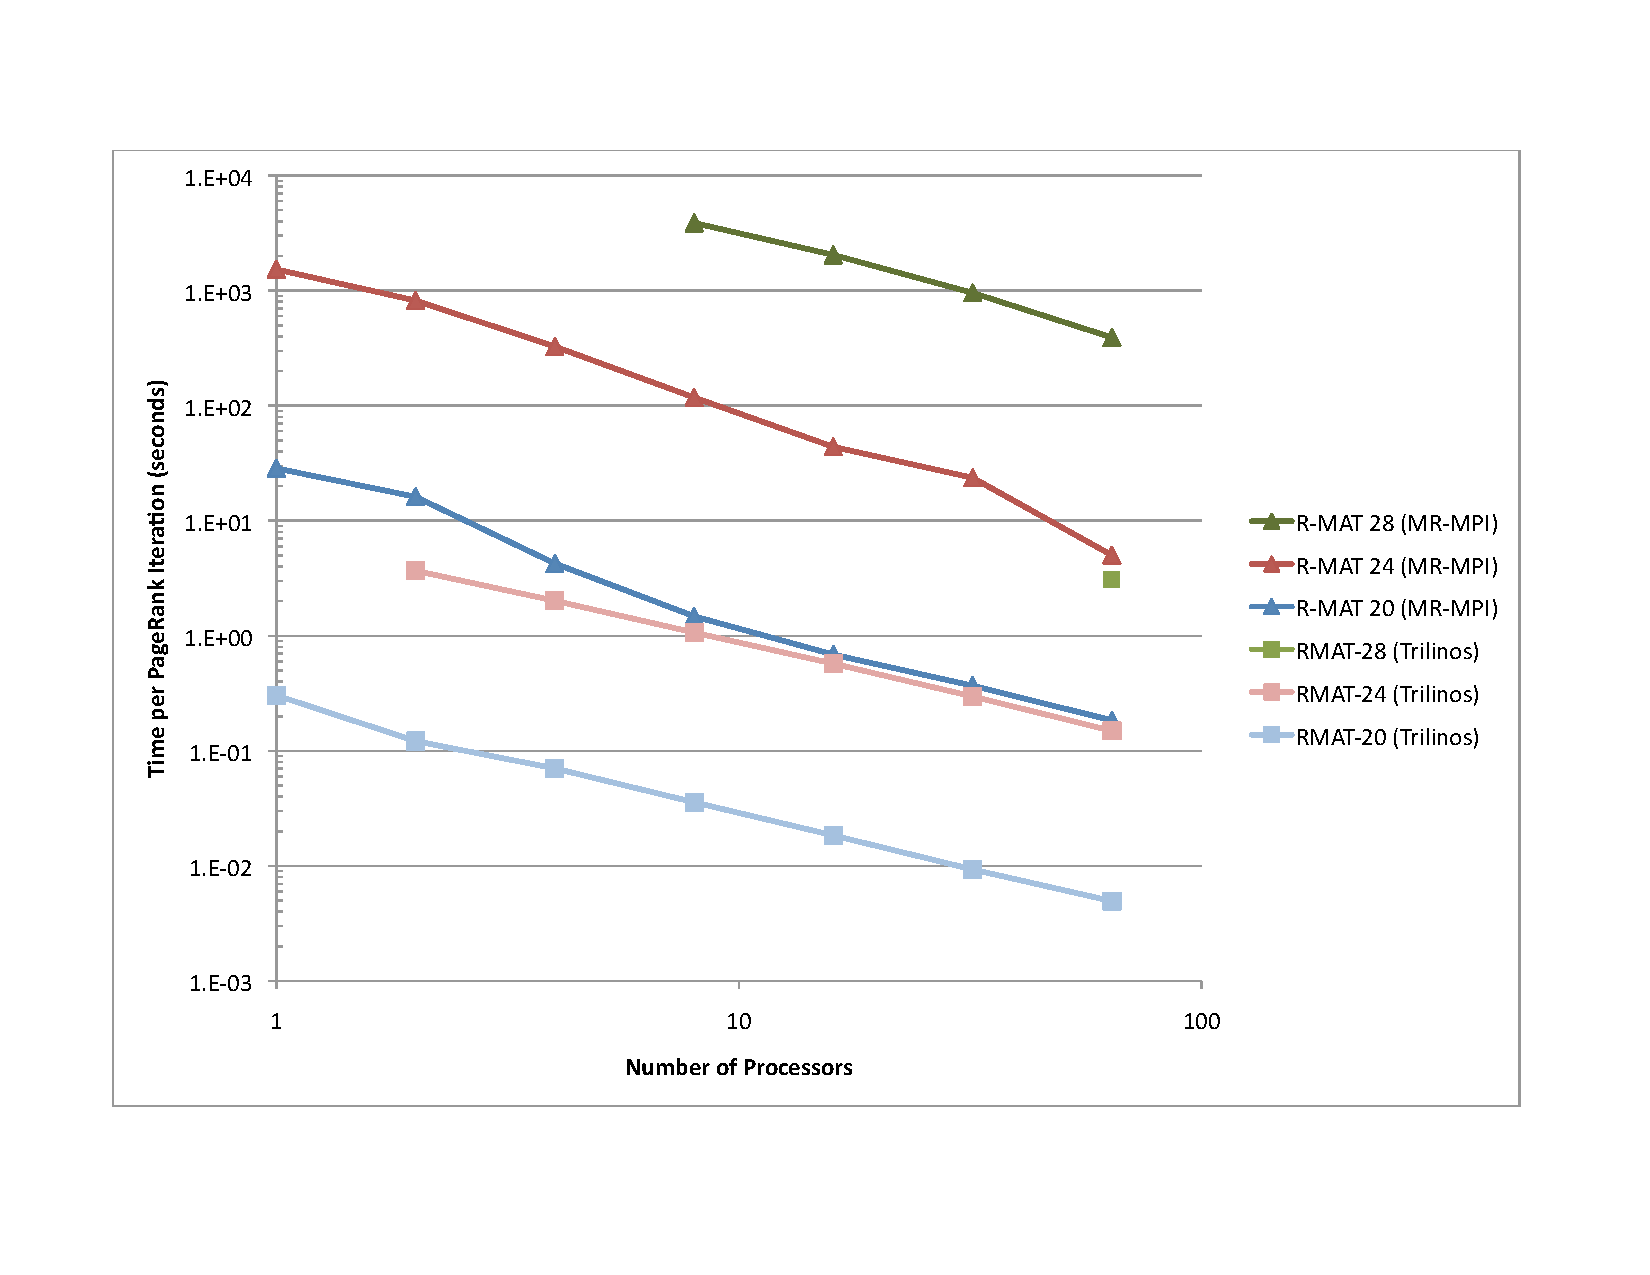
\includegraphics[width=\textwidth]{fig_pagerank.pdf}
\caption{Comparison of PageRank implementations using 
MR-MPI (Figure~\ref{fig:pr2}) and 
Trilinos' matrix/vector classes on R-MAT data sets.}
\label{f:pr}
\end{figure}


A more detailed analysis of the performance of the MR-MPI PageRank 
algorithm is shown
below.  We perform the analysis using RMAT-20, which is small enough to
fit in memory and thus does not need out-of-core operations, and RMAT-28,
which requires out-of-core operation in MR-MPI.  Table~\ref{table:prdetail}
shows the amount of time spent in each step of Figure~\ref{fig:pr2} for 
the MR-MPI implementation and the Trilinos implementation.  We see that for
both implementation, the matrix-vector multiplication (Step 2) is the most
costly step.  However, the MR-MPI algorithm is consistently slower than
the Trilinos implementation in each step.  This effect is more pronounced
for RMAT-28, where MR-MPI performs out-of-core operations.

\begin{table}[htb]
\begin{center}
\begin{tabular}{|l|r|r|r|r|}
\hline 
& \multicolumn{2}{|c|}{RMAT-20} & \multicolumn{2}{|c|}{RMAT-28} \\
& MR-MPI & Trilinos & MR-MPI & Trilinos  \\
\hline
Step 1 (Compute adjustment) & 0.0203 & 0.00030 & 17.53 & 0.0838 \\
Step 2 (Multiply $A^T x$) & 0.1377 & 0.00455 & 341.26 & 2.9239 \\
Step 3 (Apply adjustment) & 0.0015 & 0.00015 & 2.14 & 0.0494 \\
Step 4 (Scale $y$)  & 0.0013 & 0.00014 & 1.74 & 0.0359 \\
Step 5 (Compute residual)  & 0.0207 & 0.00014 & 21.20 & 0.0457 \\
\hline
\end{tabular}
\caption{Detailed execution times (in seconds) per PageRank iteration
for each stage of the algorithm
in Figure~\ref{fig:pr2} using MR-MPI and Trilinos.}
\label{table:prdetail}
\end{center}
\end{table}


To understand where MR-MPI spends its effort during the PageRank computation,
we break down the operation times further for the most expensive 
step of the PageRank computation, Step 2; the results are in 
Table~\ref{table:prdetail2}.
In the table, we divide the collate operation into its
two parts:  an aggregate that involves parallel communication and a convert
that gathers local key-value pairs with matching keys into a key-multivalue
pair.  All interprocessor communication occurs in the aggregate operation.
While the time spent in aggregate is significant, it is small compared to
the time spent in the two convert operations.  When out-of-core operations
are used for RMAT-28, the communication cost in the aggregate operation is
a smaller percentage of total time for Step 2, 
as other data manipulation operations such as convert and add 
take a relatively larger percentage of the total time.
Further experimentation
is needed to determine whether reorganizing the MapReduce data 
(as described in Section~\ref{subsec:graph_pagerank}) would reduce the
execution time of Step 2.  Organizing the data such that both the matrix
$A$ and vectors $x$ and $y$ are in the same MapReduce object would eliminate
the copy and add functions, as well as the first convert.  However, to update
the $y$ values at the completion of Step 2, either an additional convert
or an aggregate with greater amounts of data would be needed.

\begin{table}[htb]
\begin{center}
\begin{tabular}{|l|r|r|}
\hline 
PageRank Step 2 & RMAT-20 & RMAT-28 \\
\hline
Copy $x$ to $y$                       &  1.1\% &  0.4\%\\
Add $A$ to $y$                        &  3.0\% & 14.3\% \\
Convert $y$                           & 23.5\% & 43.6\% \\
Reduce $y$                            &  7.7\% &  5.8\% \\
Aggregate $y$ (first part of collate) & 24.9\% &  6.8\% \\
Convert $y$ (second part of collate)  & 38.2\% & 27.4\% \\
Reduce $y$                            &  1.6\% &  1.7\% \\
\hline
\end{tabular}
\caption{Percentage of execution time in each operation of Step 2 of the MR-MPI 
PageRank algorithm in Figure~\ref{fig:pr2}.}
\label{table:prdetail2}
\end{center}
\end{table}

Similarly, in Table~\ref{table:prdetail5}, we show the execution times 
required for each operation in Step 5 of Figure~\ref{fig:pr2}, the 
residual computation.  Clearly the time to convert key-value pairs to 
key-multivalues dominates this computation.  Reorganization of the vectors
$x$ and $y$ into a single MapReduce object (as described in 
Section~\ref{subsec:graph_pagerank}) would benefit this step of the computation,
as the add, convert, and reduce operations could be replaced by a single 
map operation, with execution time comparable to the vector-scaling operation
in Step 4.

\begin{table}[htb]
\begin{center}
\begin{tabular}{|l|r|r|}
\hline 
PageRank Step 5 & RMAT-20 & RMAT-28 \\
\hline
Add $y$ to $x$ &  2.2\% &  9.8\% \\
Convert $x$    & 95.1\% & 84.9\% \\
Reduce $x$     &  2.5\% &  5.3\% \\
MPI\_Allreduce &  0.2\% &  0.0\% \\
\hline
\end{tabular}
\caption{Percentage of execution time in each operation of Step 5 of the MR-MPI 
PageRank algorithm in  Figure~\ref{fig:pr2}.}
\label{table:prdetail5}
\end{center}
\end{table}
%This result is
%due to two factors: ({\it i}) a higher volume of communication in the
%MapReduce implementation (which comunicates one datum per graph edge
%in each iteration), compared to the Trilinos implementation which only
%communicates a volume of data proportional to the number of vertices,
%and ({\it ii}) out-of-core operations in MR-MPI were performed because
%of the page-size restriction, while all Trilinos operations were
%performed in-core.  
%

\subsection{Triangle finding results}

In Figure~\ref{f:tri}, we show the performance of the triangle finding
algorithm (Figure~\ref{fig:tri}).  Execution times for this algorithm
were too large to allow the problem to be easily run with RMAT-28 on
our cluster.  Parallel efficiencies for RMAT-20 ranged from 80\% to
140\%; for RMAT-24, they ranged from 50\% to 120\%.

%Comparisons with an MTGL implementation on the 
%Cray XMT give mixed results.  When MR-MPI uses the least file I/O for 
%out-of-core operations (e.g., RMAT-20 on 32 and 64 processors), it 
%outperforms the MTGL implementation.  However, when significant out-of-core
%operations are needed (e.g., for RMAT-24), the MTGL implementation is faster.

\begin{figure}[htb]
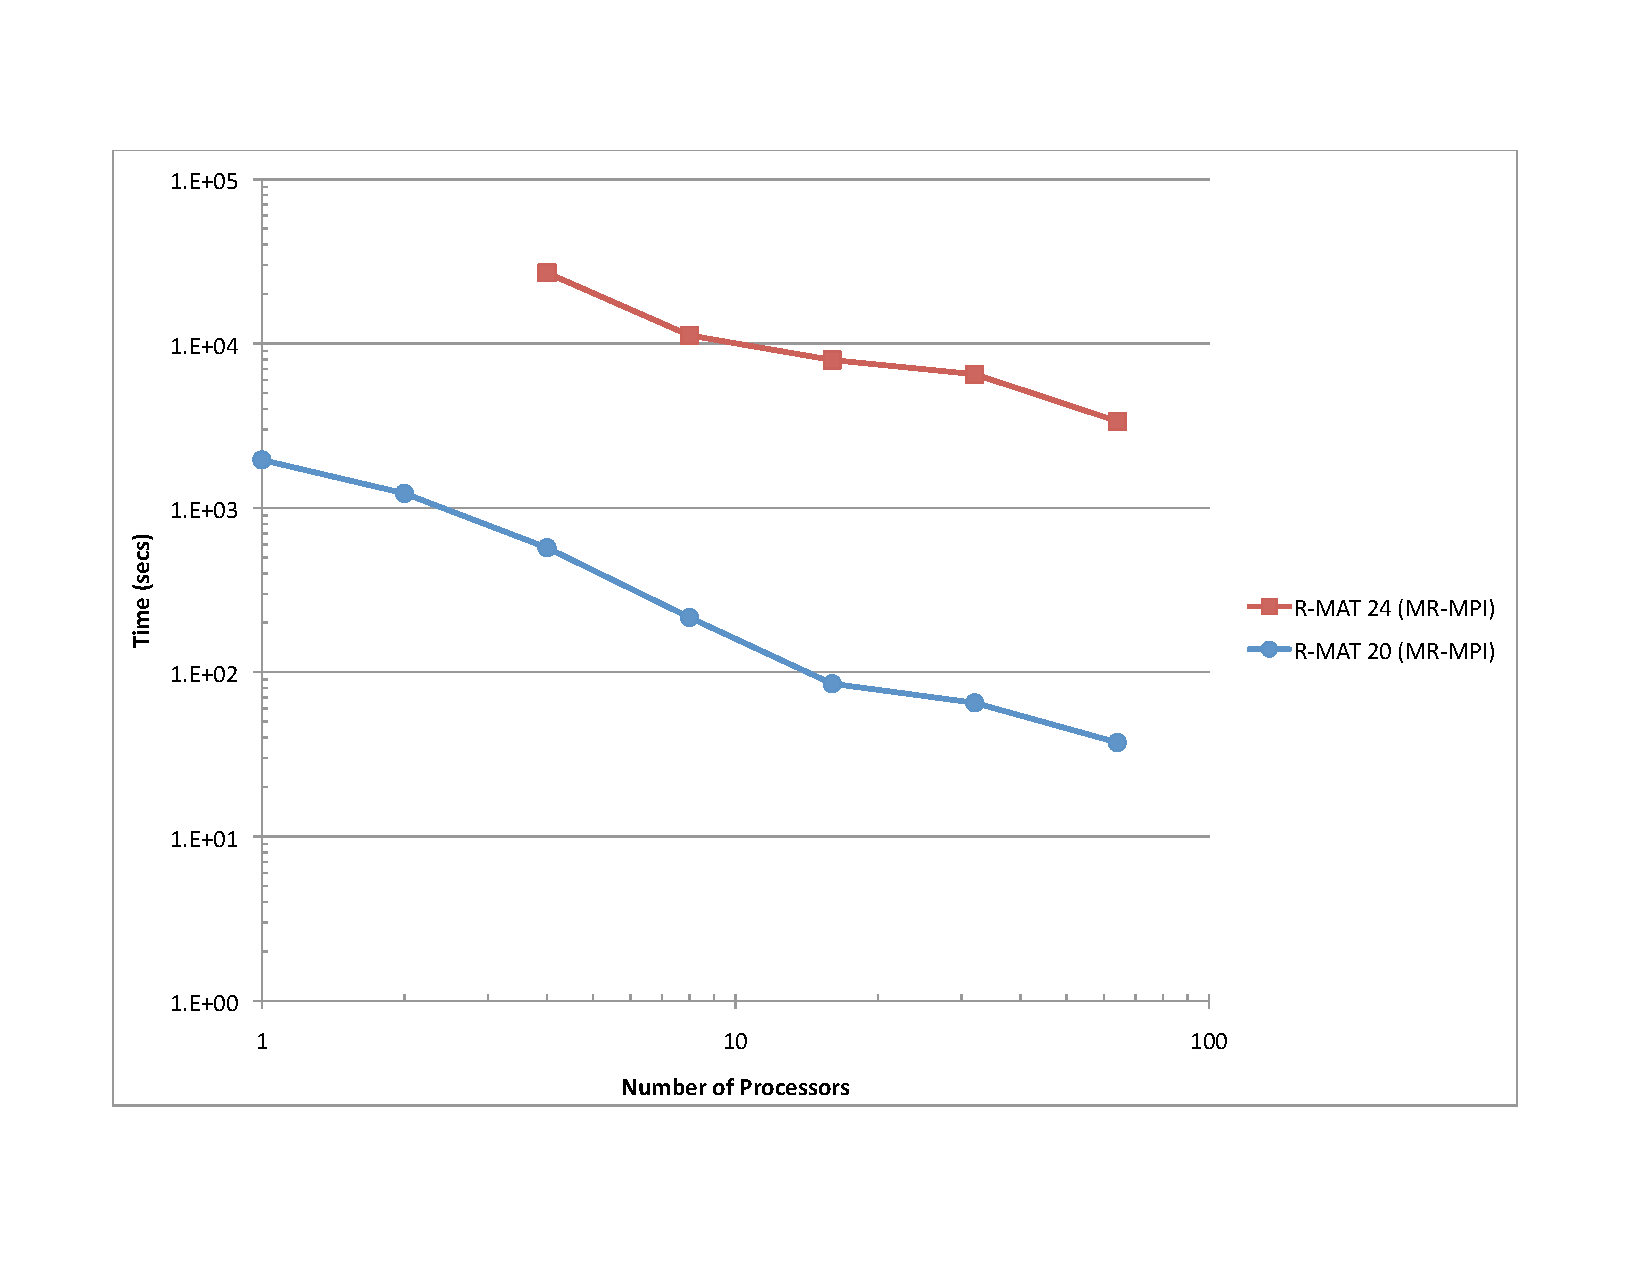
\includegraphics[width=\textwidth]{fig_tri.pdf}
\caption{Performance of the MR-MPI triangle-finding algorithm
(Figure~\ref{fig:tri}).}
\label{f:tri}
\end{figure}

\subsection{Connected Components}

In Figure~\ref{f:cc}, we show the performance of the connected
component identification algorithm (Figure~\ref{fig:cc}).  A
comparison is made with a hybrid ``Giant Connected Component''
implementation using both Trilinos and MR-MPI.  Power law graphs often
have one or two very large components and many very small components.
The hybrid algorithm exploits this feature of the data by using
inexpensive breadth-first search (BFS) from the vertex with highest
degree to identify the largest components, followed by a more
expensive algorithm to identify the small components in the remainder
of the graph.  In our hybrid implementation, we intially perform
matrix-vector multiplications in Trilinos to perform a BFS, finding
components that include (in total) 70\% or more of the vertices.  We
then apply our MR-MPI algorithm to the remaining graph to identify the
small components.  This hybrid approach is quite effective, reducing
the execution time to identify all components of RMAT-20 and RMAT-24
by 80-99\%, as shown in Figure~\ref{f:cc}.  The benefit of MR-MPI is
seen, however, for RMAT-28, where the graph is too large to fit into
memory, and thus Trilinos cannot perform the initial BFS for our
hybrid algorithm.

\begin{figure}[htb]
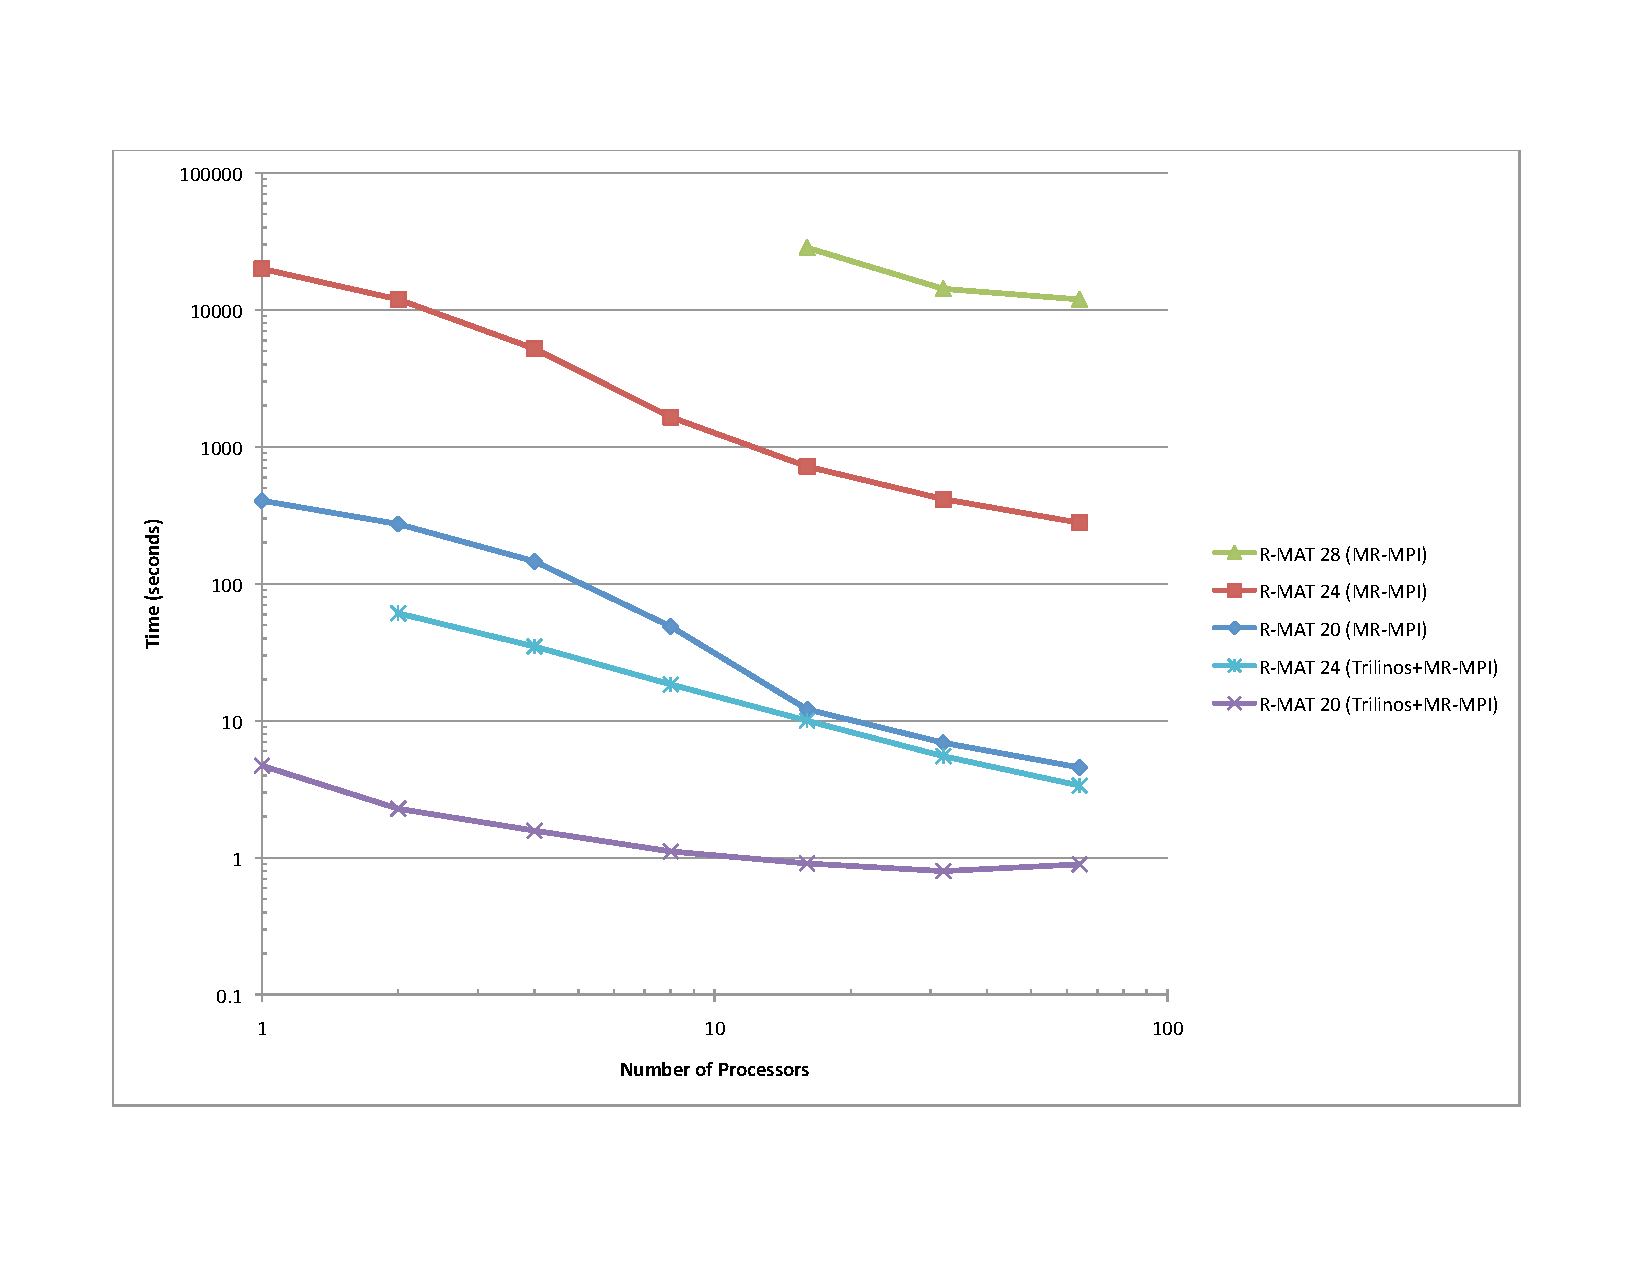
\includegraphics[width=\textwidth]{fig_cc.pdf}
\caption{Performance of the MR-MPI connected components algorithm (Figure~\ref{fig:cc}) compared with a hybrid ``Giant Connected Component'' algorithm based
on Trilinos.}
\label{f:cc}
\end{figure}

\subsection{Maximally independent set results}

The execution times for the maximal independent set algorithm
(Figure~\ref{fig:luby}) are shown in Figure~\ref{f:luby}.  Like the
R-MAT generation results, superlinear speed-up of the algorithm occurs
for RMAT-20 and RMAT-24, as more of the graph fits into processor
memory and less file I/O is needed.  For RMAT-28, the algorithm
requires significant out-of-core operations. In this case, parallel
efficiency is nearly perfect going from 8 to 64 processors.

\begin{figure}[htb]
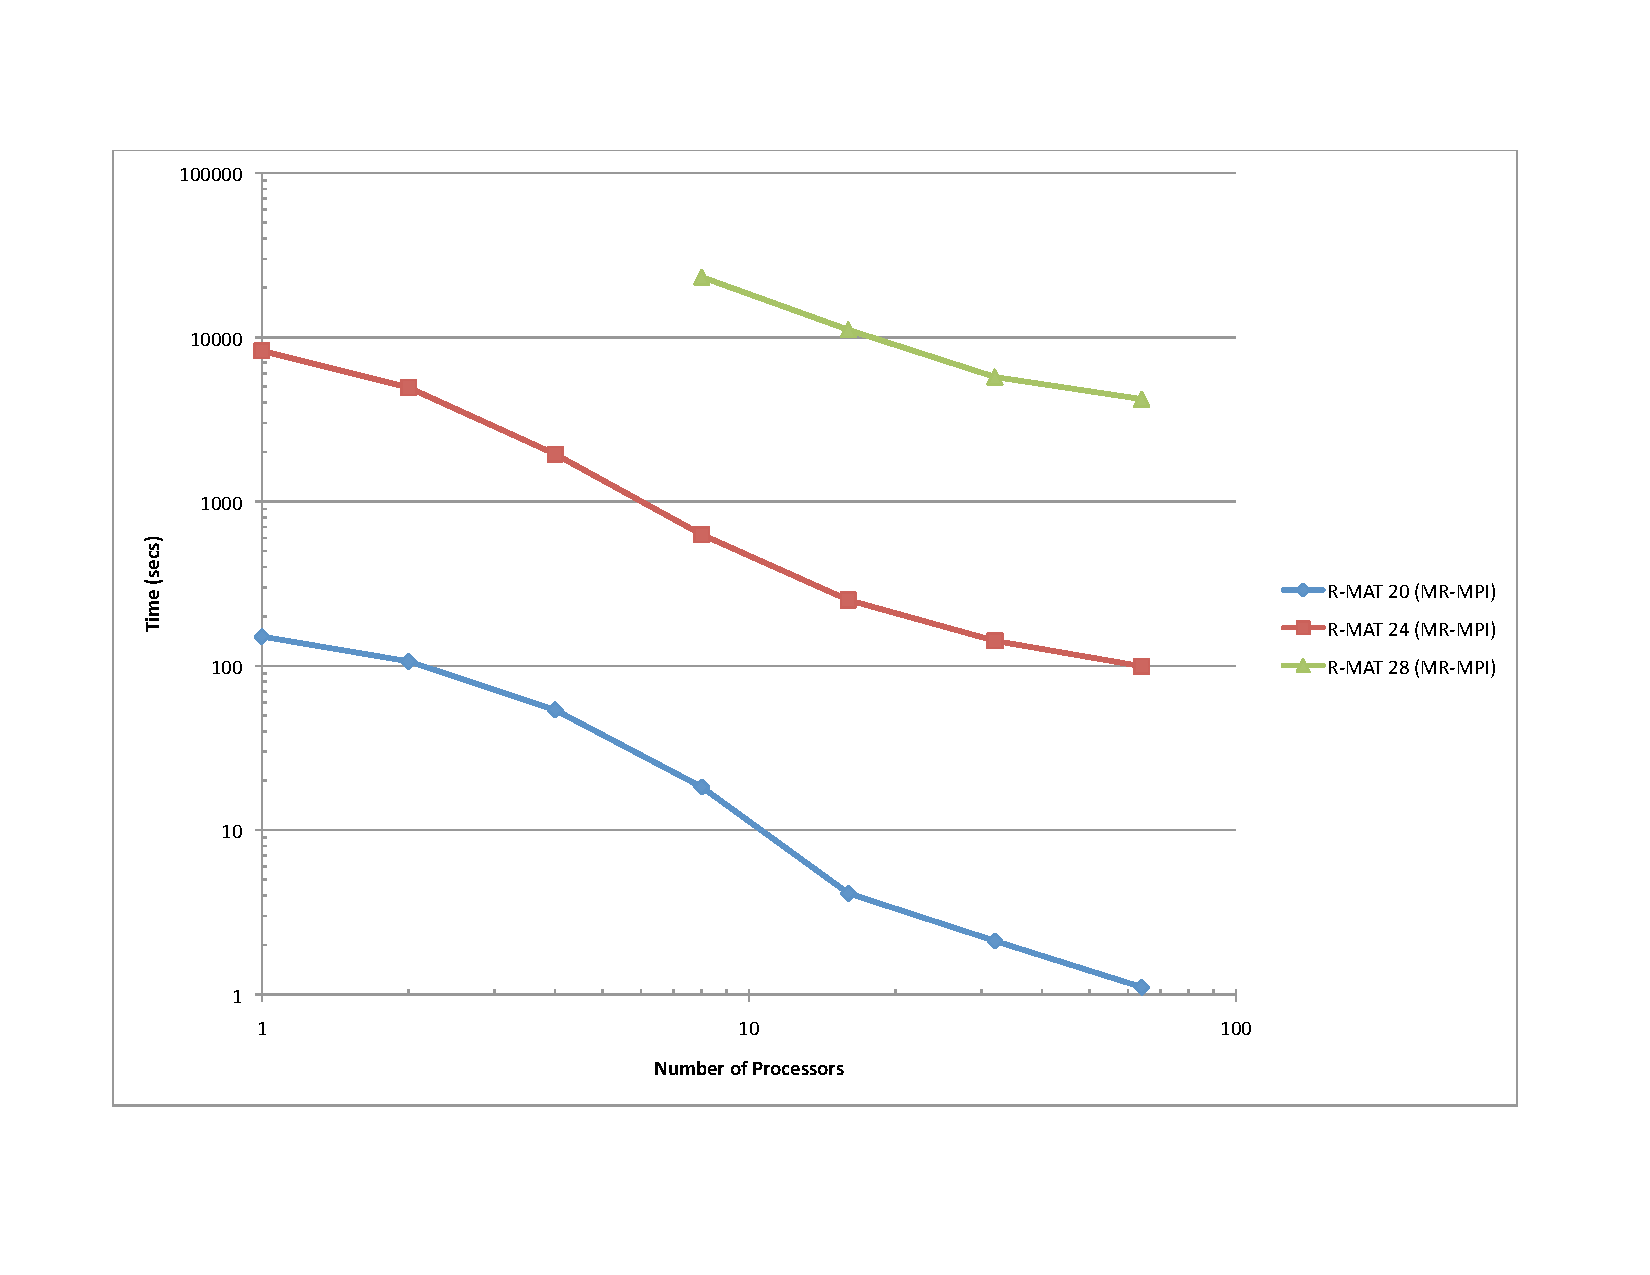
\includegraphics[width=\textwidth]{fig_luby.pdf}
\caption{Performance of the MR-MPI maximal independent set algorithm (Figure~\ref{fig:luby}).}
\label{f:luby}
\end{figure}

\subsection{Single-source shortest path results}

The execution times for the single-source shortest path algorithms
(Figures~\ref{fig:sssp} and \ref{fig:sssp2}) are shown in
Figure~\ref{f:sssp}.  The results show the benefit of using the
enhanced algorithm, providing at least a 17\% (and often greater)
reduction in execution time due to reduced communication; only the
updated distances are communicated throughout most of the enhanced
algorithm.  However, the execution times are still large compared to
multi-threaded implementations; for example, Madduri et
al.~\cite{Madduri07} report execution times of only 11 seconds on 40
processors for a multithreaded implementation on a Cray MTA-2 (the
predecessor of the XMT) on graphs with one billion edges.

\begin{figure}[htb]
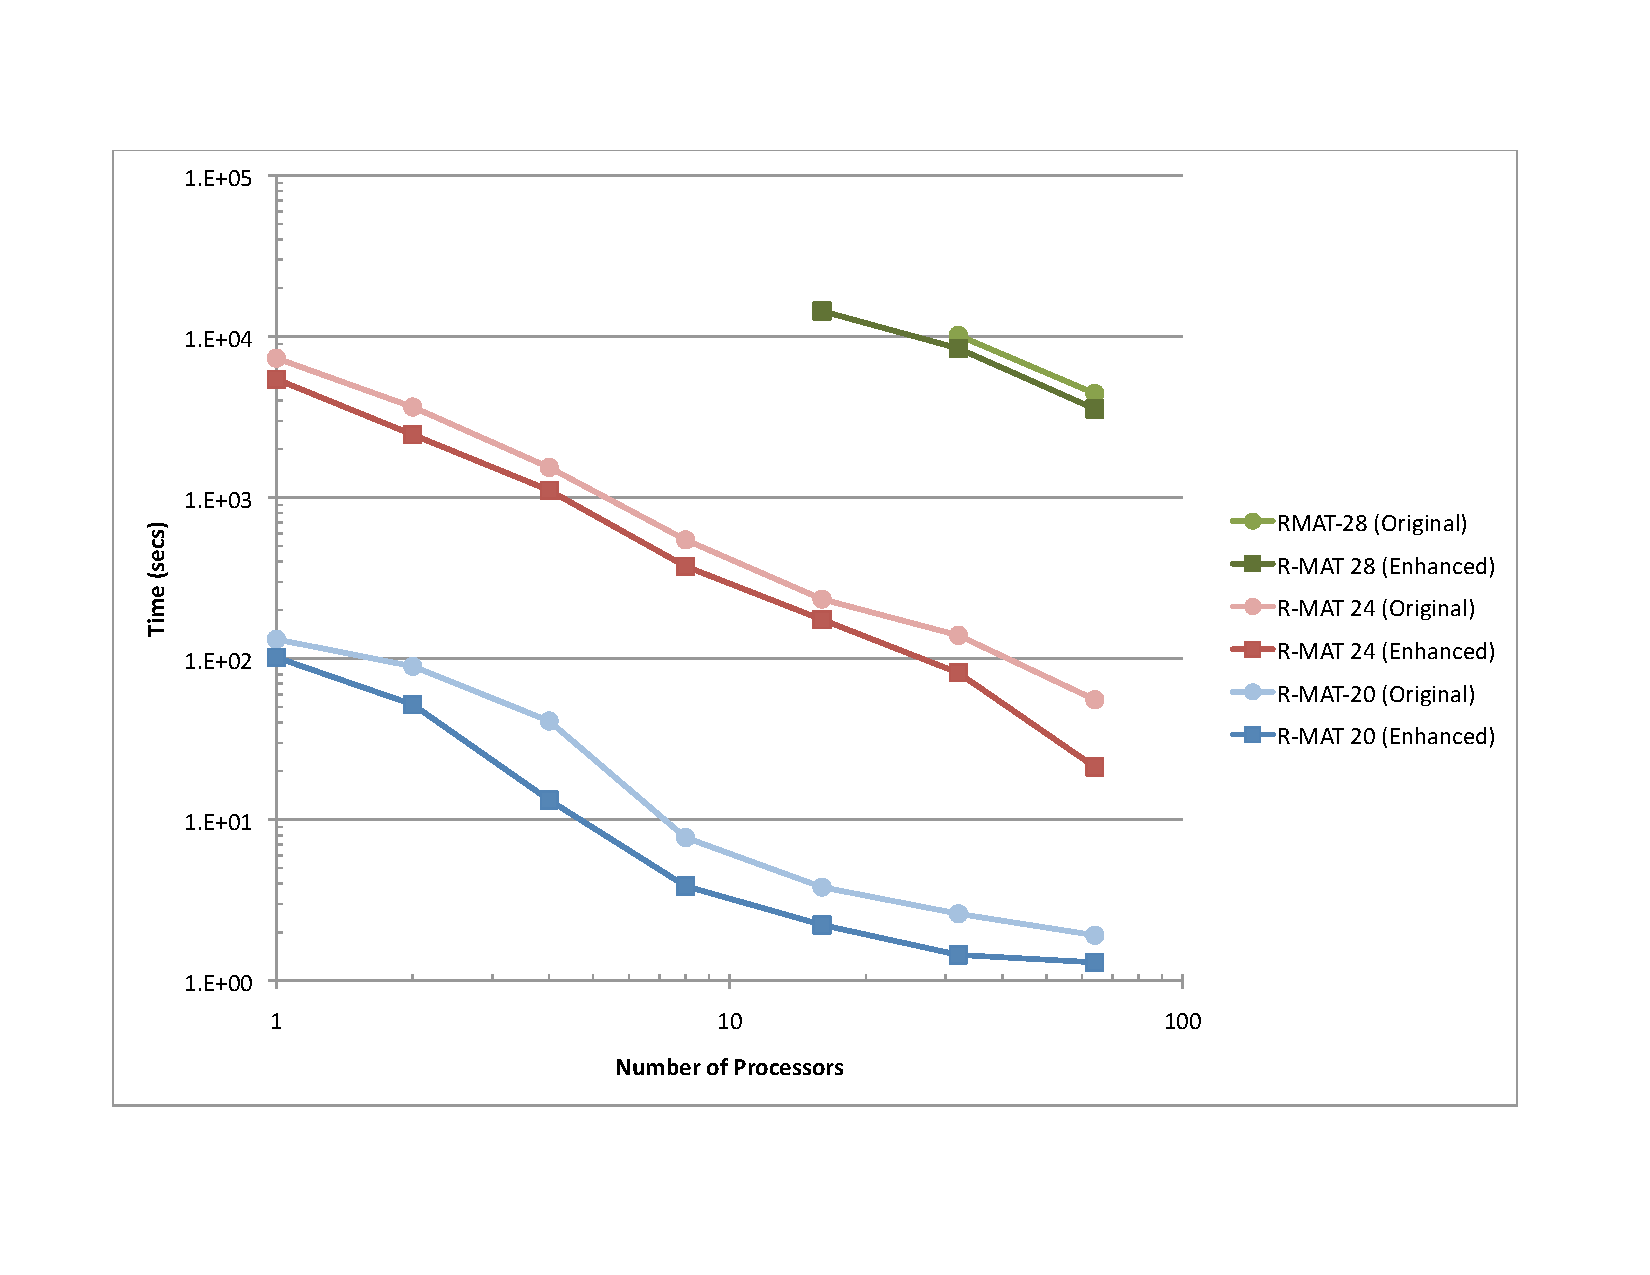
\includegraphics[width=\textwidth]{fig_sssp.pdf}
\caption{Execution times for SSSP using MR-MPI with R-MAT matrices.  
Both the original algorithm (Figure~\ref{fig:sssp}) and the enhanced 
algorithm (Figure~\ref{fig:sssp2}) are included.}
\label{f:sssp}
\end{figure}

To compare our MR-MPI implementation with a wider set of algorithms,
we performed experiments comparing MR-MPI, Hadoop, PBGL (Parallel
Boost Graph Library)~\cite{PBGL} and a multi-threaded implementation
on the Cray XMT using two web graphs: {WebGraphA} with 13.2M vertices
and 31.9M edges, and {WebGraphB} with 187.6M vertices and 531.9M
edges.  In Figure~\ref{f:ssspA}, we show execution times for the SSSP
algorithm using {WebGraphA}.  Like our MR-MPI implementation, the
Hadoop implementation is a Bellman-Ford-style~\cite{Bellman58,Ford62}
algorithm.  The XMT and PBGL implementations are based on
delta-stepping~\cite{MeyerSanders98}, and do not require full
iterations over the entire edge list to advance a breadth-first
search.  We observe that the MR-MPI implementation runs in less time
than the Hadoop implementation, but requires significantly more time
than the XMT and PBGL implementations.  In experiments with
{WebGraphB}, the benefit of the enhanced algorithm
(Figure~\ref{fig:sssp2}) is clearly shown, with a 40\% reduction in
execution time compared to the original SSSP algorithm
(Figure~\ref{fig:sssp}).  But the Bellman-Ford-style iterations are
especially harmful to the MR-MPI and Hadoop implementations for
{WebGraphB}, which required 110 iterations to complete; execution
times for this data set are shown in Table~\ref{t:ssspB}.

\begin{figure}[htb]
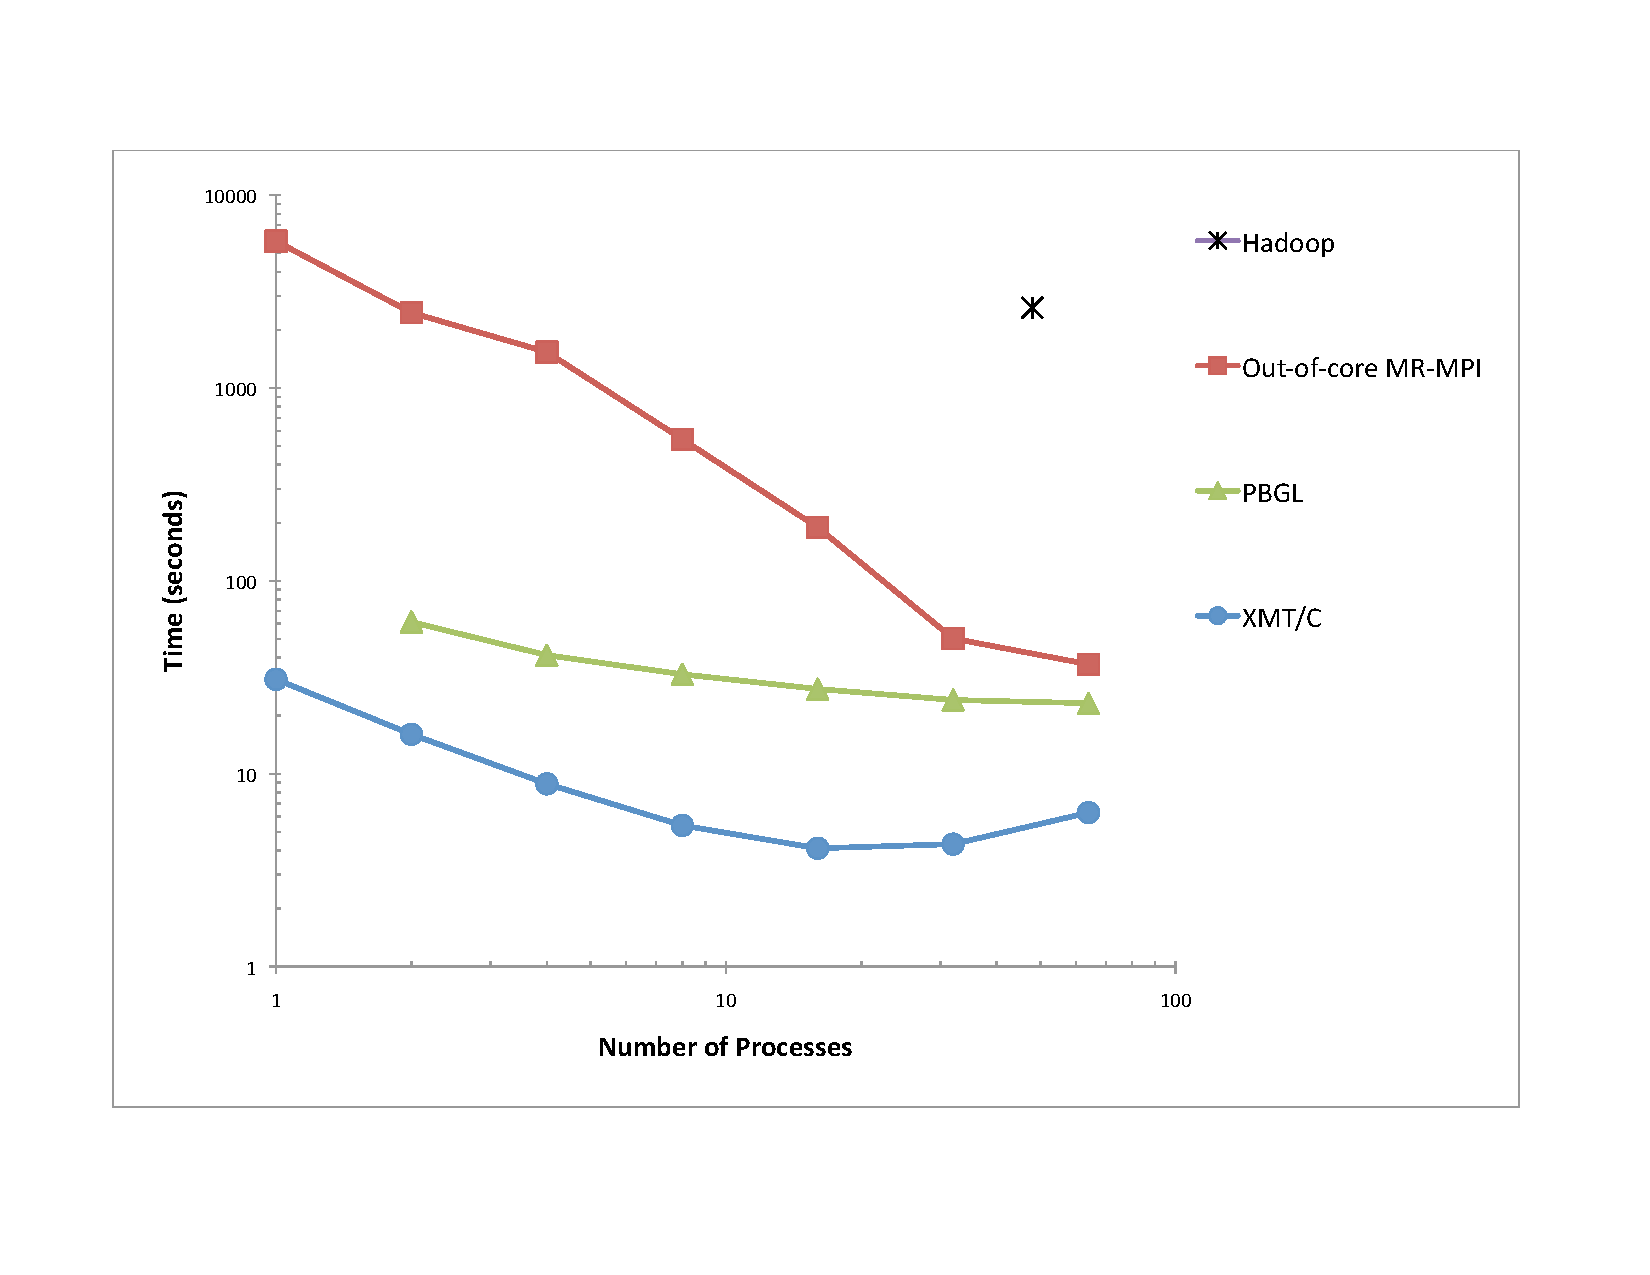
\includegraphics[width=\textwidth]{fig_ssspA.pdf}
\caption{SSSP using MR-MPI for WebGraphA with
13.2M vertices and 31.9M edges.  Runtimes using Hadoop and PBGL
are also shown.}
\label{f:ssspA}
\end{figure}

\begin{table}
\begin{center}
\begin{tabular}{|l|c|r|}
\hline
Implementation & Number of Processes & SSSP Execution Time \\
\hline
Hadoop & 48  & 38,925 secs.\\
MR-MPI original (Figure~\ref{fig:sssp}) & 48 &  13,505 secs.\\
MR-MPI enhanced (Figure~\ref{fig:sssp2}) & 48 &  8,031 secs.\\
XMT/C  & 32 &  37 secs.\\
%Out-of-core MR-MPI & 96 &   8,358 secs.\\
%Out-of-core MR-MPI & 64 &  12,882 secs.\\
%Out-of-core MR-MPI & 100 &  6,280 secs.\\
\hline
\end{tabular}
\caption{Execution times for SSSP with {WebGraphB}.}
\label{t:ssspB}
\end{center}
\end{table}

\subsection{Scalability to large numbers of processors}

Finally, we demonstrate the scalability of our MR-MPI library to large
numbers of processors.  The library was used on Sandia's Redstorm and
Thunderbird parallel computers.  Redstorm is a large Cray XT3 with 2+
{GHz} dual/quad-core AMD Opteron processors and a custom interconnect
providing 9.6 GB/s of interprocessor bandwidth.  Thunderbird is a
large Linux cluster with 3.6 {GHz} dual-core Intel EM64T processors
connected by an Infiniband network.  Because these systems do not have
local disks for each processor, we selected a data set and page sizes
that fit in memory, so out-of-core operations were not needed.  For
these experiments, we used an R-MAT data set with with $2^{25}$
vertices and $2^{28}$ edges, with parameters given in
Table~\ref{t:rmat}.  We ran both the PageRank and Connected Components
algorithms.

\begin{table}
\begin{center}
\begin{tabular}{|l|c|c|c|c|c|c|c|}
\hline
Data & R-MAT  & R-MAT  & R-MAT  & R-MAT  & \# of    & \# of & Maximum \\
Set  & a      & b      & c      & d      & vertices & edges & vertex degree\\
\hline
nice  & 0.45 & 0.15 & 0.15 & 0.25 & $2^{25}$ & $2^{28}$ & 1108 \\
nasty & 0.57 & 0.19 & 0.19 & 0.05 & $2^{25}$ & $2^{28}$ & 230,207\\
\hline
\end{tabular}
\caption{Characteristics of R-MAT input data for PageRank and Connected
Components scalability experiments.}
\label{t:rmat}
\end{center}
\end{table}

Figure~\ref{f:prbig}, shows the performance of the various PageRank
implementations on distributed memory and multi-threaded
architectures.  The MR-MPI and Trilinos implementations are described
in Sections~\ref{subsec:graph_pagerank}
and~\ref{subsec:results_pagerank}, respectively.  In the
multi-threaded MTGL implementation, rank propagates via adjacency list
traversal in a compressed sparse-row data structure.  To maintain its
scalability, code must be written so that a single thread spawns the
loop that processes all in-neighbors of a given vertex; this detail
enables the compiler to generate hotspot-free code.

The MR-MPI implementation demonstrated good scalability up to 1024
processors; however, as before, it required an order-of-magnitude more
execution time than the matrix-based implementations on Redstorm.  The
distributed memory matrix-based implementations are competitive with
the multi-threaded implementation in MTGL on the Cray XMT.

\begin{figure}[htb]
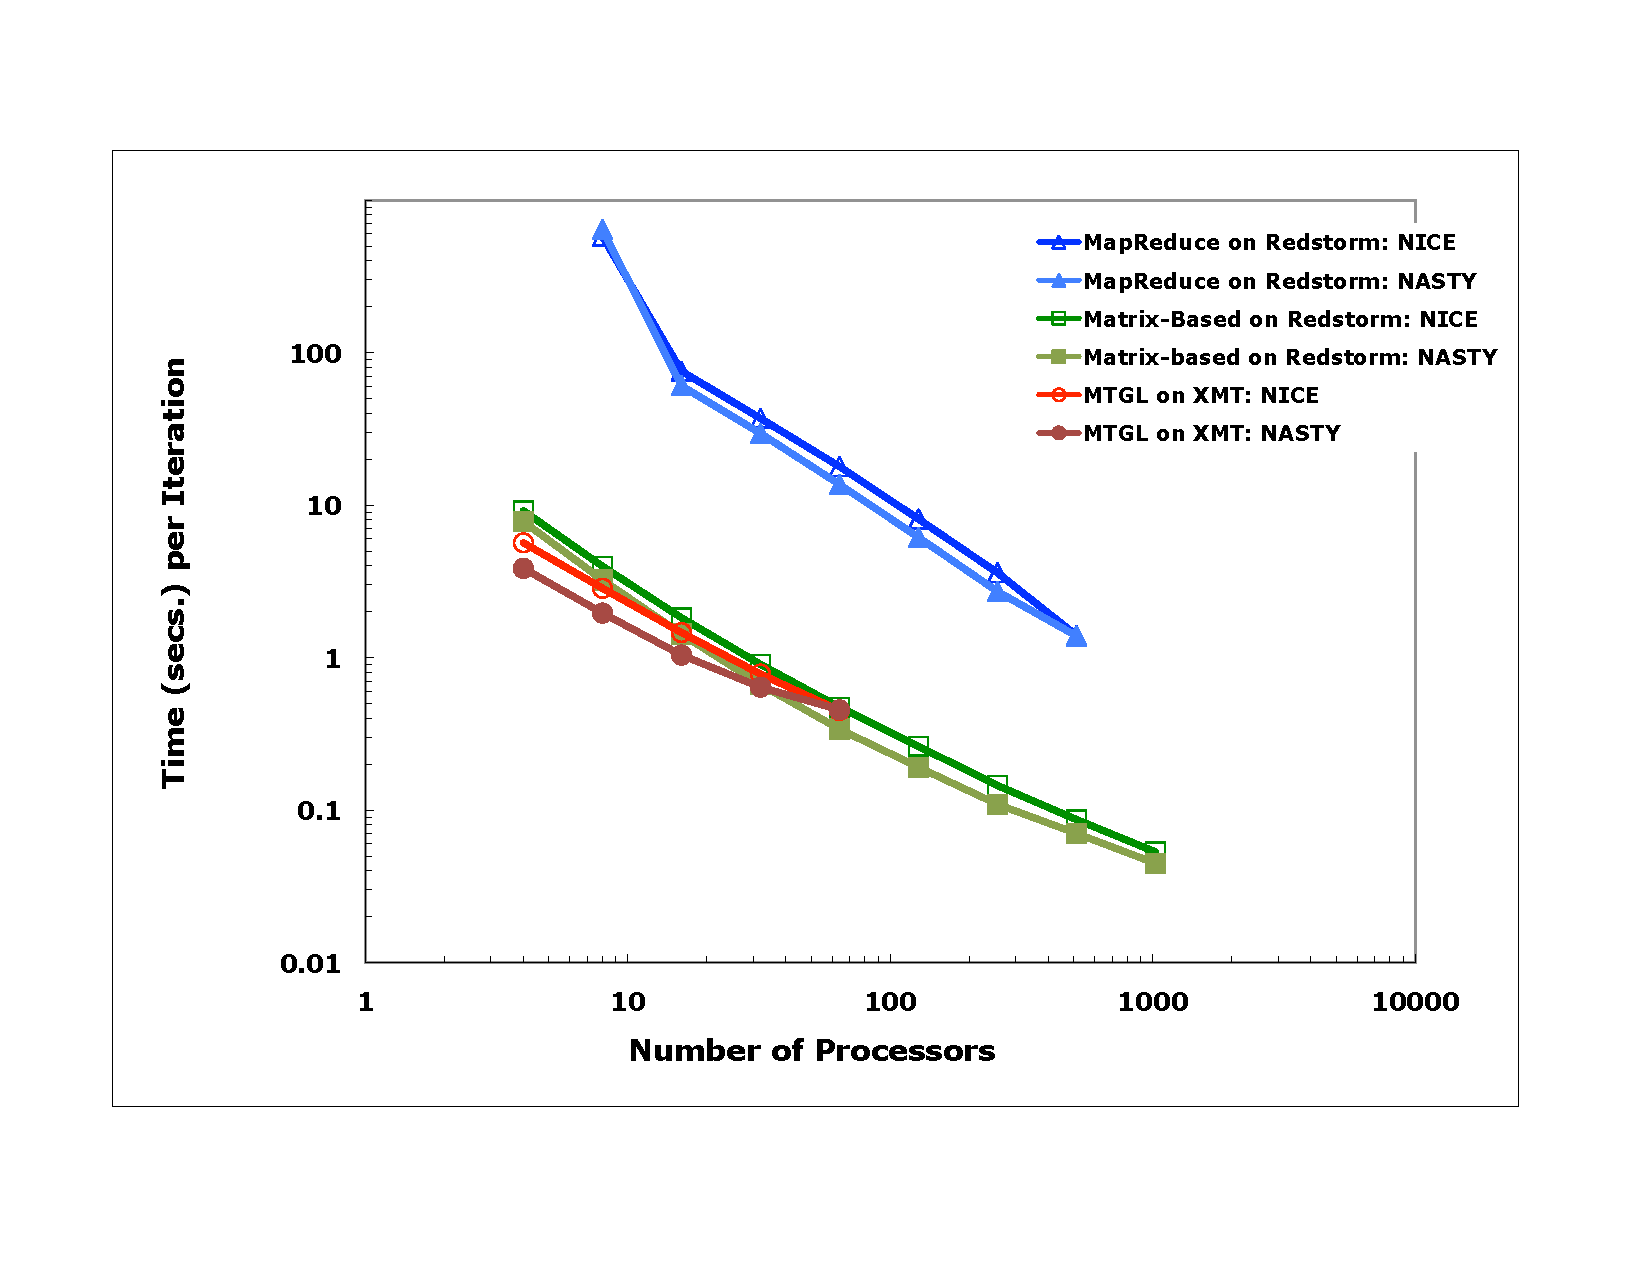
\includegraphics[width=\textwidth]{fig_pagerank_big.pdf}
\caption{Scalability comparison of PageRank using MapReduce (MR-MPI),
matrix-based (Trilinos), and multi-threaded (MTGL) implementation on
the R-MAT data sets in Table~\ref{t:rmat}.}
\label{f:prbig}
\end{figure}

Similar results were obtained for the Connected Components algorithm,
as shown in Figure~\ref{f:ccbig}.  As with PageRank, the MR-MPI
implementation showed good scalability up to 1024 processors, but
required significantly more time than the hybrid algorithm using
Trilinos and MR-MPI or the MTGL algorithm.

\begin{figure}[htb]
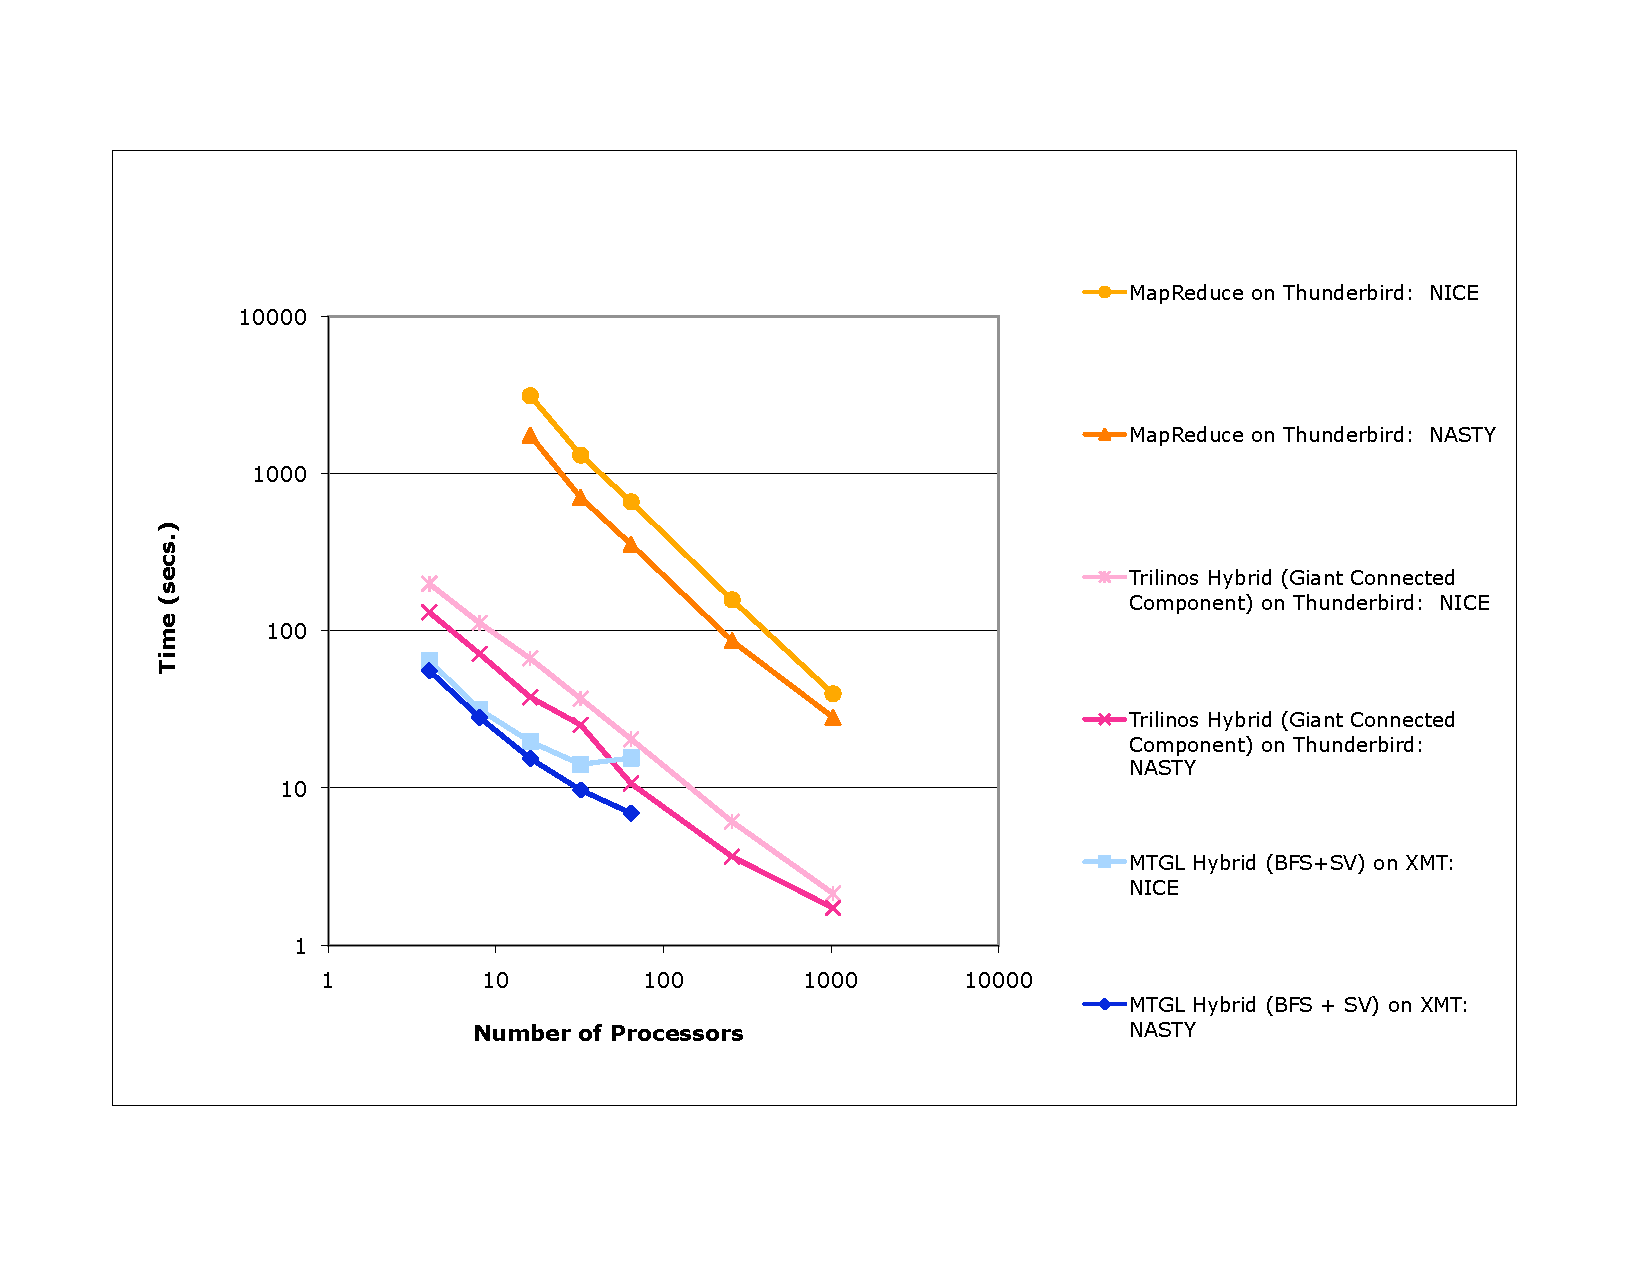
\includegraphics[width=\textwidth]{fig_cc_big.pdf}
\caption{Scalability comparison of Connected Components algorithms using 
MapReduce (MR-MPI),
matrix-based/MapReduce hybrid (Trilinos/MR-MPI), and MTGL implementations
on the R-MAT data sets in Table~\ref{t:rmat}.}
\label{f:ccbig}
\end{figure}

